% !TeX encoding = UTF-8

\chapter{ANÁLISE DOS RESULTADOS}\label{ch:resultados}
Este capítulo tem como finalidade apresentar os resultados obtidos através das implementações demonstradas no Capítulo 5.

\section{ANÁLISE DAS SÉRIES UTILIZADAS}
Após a implementação do modelo da RNA, através dos conjuntos de dados coletados, faz-se necessário avaliar como a respectiva técnica se comportou. Tendo isso em vista, a mesma foi aplicada em função do objetivo principal do trabalho, que é medir a capacidade de precisão de acerto no valor de abertura das ações. Portanto, foi elaborada, de forma independente, uma análise de eficácia do modelo para o cenário de cada empresa utilizada no presente trabalho. É importante ressaltar que os modelos foram implementados levando em consideração todos os \textit{scripts}, métodos e ferramentas utilizadas no capítulo anterior.

\subsection{Aplicação da rede na Intel Corporation}
A rede da Intel Corporation foi treinada com o objetivo de capturar o maior nível de variação possível dos dados, visando mapear um maior conjunto de padrões e, assim, responder de forma eficiente à dados dispersos através de uma boa capacidade de generalização. Tendo isso em vista, o período de treinamento preparado foi de 09/04/2001 até 21/08/2017, totalizando 4117 registros.

Para o presente caso foram construídos dois cenários de simulação, buscando obter um parâmetro de ciclos de treinamento adequado ao modelo de dados utilizado. As métricas definidas para análise, a partir destes ciclos de treinamento, são: o comportamento da função de custo que compõem o modelo (erro quadrático médio, EQM) e a margem de erro dos valores resultantes da rede, no período de 23/08/2017 a 31/08/2017, em relação aos valores reais. Os parâmetros utilizados foram: 200 e 1000 iterações.

\subsubsection{Treinamento com 200 Iterações}	
A ideia de executar o treinamento com uma quantidade baixa de iterações, é feita com o intuito de proporcionar um treinamento mais rápido e com resultados significativos, levando em consideração as características especificas do modelo de dados. Portanto, para quantificar como ocorreu o processo de treinamento, basta multiplicar o número de iterações (200) com o número de registros de testes (4117), resultando em um total de 823.400 exemplos calculados pela rede. O Gráfico 8 demonstra, de acordo com a quantidade de ciclos, a variação do EQM no primeiro cenário de teste com 200 iterações.
\begin{grafico}[h]
	\centering
	\fbox{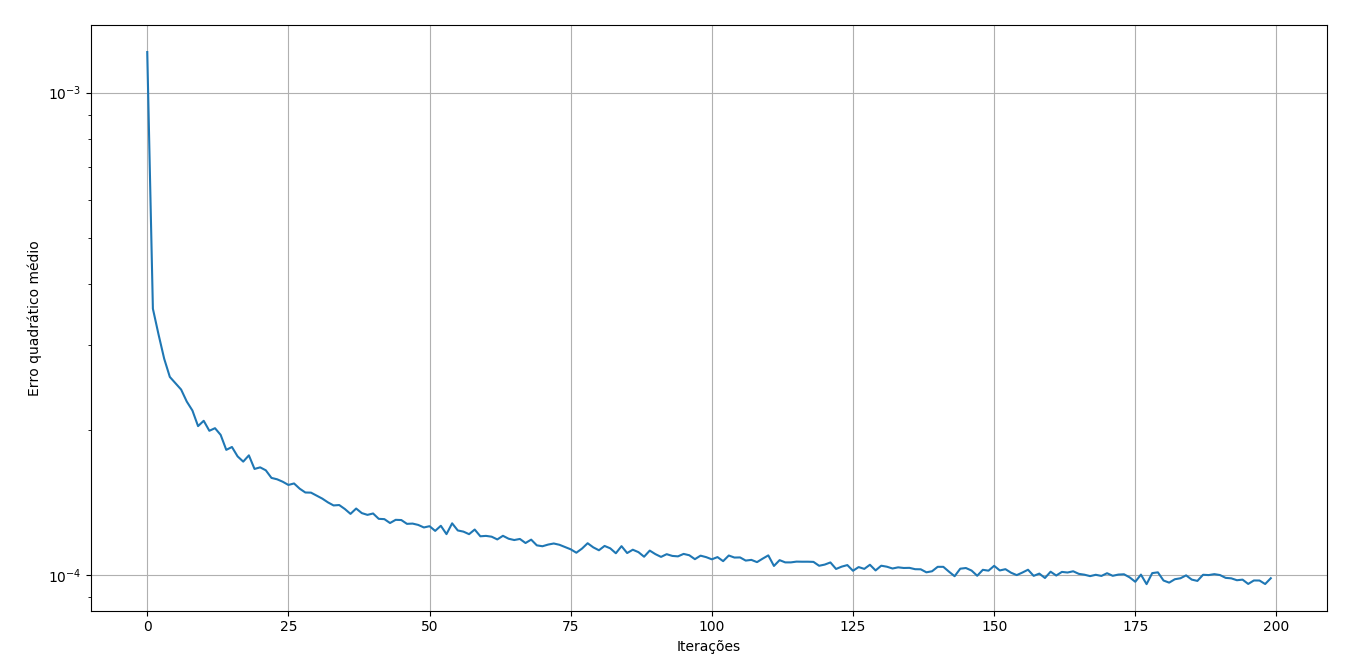
\includegraphics[width=1\textwidth]{erro_intel_primeiro}}
	\caption{Decaimento do EQM no treinamento da rede}
	\fonte{Elaborado pelo autor}
	\label{lingua}
\end{grafico}

O EQM iniciou-se, na primeira iteração, com um erro percentual de 0.00248996652176 e, após o término das 200 épocas de treinamento, conclui-se com um erro percentual de 9.44359025338.$10^{-05}$. Analisando o gráfico, pode-se observar que os valores tiveram um decaimento constante até a iteração de número 125, enquanto que, nas 75 iterações posteriores, manteve os valores dos erros aproximados. Esta queda constante nas iterações iniciais está diretamente ligada a capacidade de aprendizado e adaptação ao modelo de dados.

Tendo em vista a variação dos erros obtidos após a primeira inicialização da rede, foi julgado necessário repetir o mesmo procedimento, visando observar o funcionamento do algoritmo de inicialização dos pesos e validar sua variação aplicada ao mesmo modelo de dados. Portanto, mais dois cenários foram executados com este objetivo. No segundo cenário, o erro foi iniciado com um percentual de 0.00102981131422 e, após o término das 200 épocas de treinamento, concluí-se com um percentual de 9.1790170623.$10^{-05}$. No terceiro cenário, o erro foi iniciado com um percentual de 0.00026991101482 e, após o término das 200 épocas de treinamento, concluí-se com um percentual de 9.49959768553.$10^{-05}$.

Analisando os três cenários, pode-se observar que apesar da rede ser iniciada com os pesos aleatoriamente, o EQM seguiu a mesma tendência para todos os casos, isso implica em uma confiabilidade maior por parte do algoritmo, pois o mesmo garante que novas inicializações, aplicadas ao mesmo modelo de dados, não resultam em valores muito distintos. Esta validação do algoritmo tem grande importância, pois com ela chega-se a definição de que os pesos iniciais da rede não precisarão, necessariamente, serem ajustados manualmente para encontrar um melhor resultado, pois aplicado ao mesmo modelo de dados, os erros seguem o mesmo padrão.

Após a verificação do comportamento do EQM e a validação do algortimo de inicialização, os testes foram iniciados com o objetivo de verificar a precisão do modelo. Na Tabela 1 são detalhados os valores do período predito.
\begin{table}[h]
\centering
\caption{Período dos dados utilizados para testes: Intel Corporation}
\vspace{0.5cm}
\begin{tabular}{>{\centering\arraybackslash}m{2cm} >{\centering\arraybackslash}m{2cm} >{\centering\arraybackslash}m{2cm} >{\centering\arraybackslash}m{2cm} >{\centering\arraybackslash}m{2cm} >{\centering\arraybackslash}m{2cm}}
\toprule
Data    & Abertura   & Alta   & Baixa   & Fechamento   & Volume\\
\midrule
23/08/2017 & 34.54 & 34.81 & 34.38 & 34.66 & 196.481,34\\
24/08/2017 & 34.70 & 34.89 & 34.55 & 34.71 & 143.018,92\\
25/08/2017 & 34.82 & 34.93 & 34.58 & 34.67 & 147.268,29\\
28/08/2017 & 34.78 & 34.80 & 34.59 & 34.65 & 207.128,76\\
29/08/2017 & 34.51 & 34.75 & 34.46 & 34.73 & 158.436,68\\
30/08/2017 & 34.75 & 34.96 & 34.63 & 34.89 & 185.650,07\\
31/08/2017 & 34.94 & 35.18 & 34.87 & 35.07 & 163.667,72\\
\bottomrule
\end{tabular}
\end{table}

Os dados demonstrados na Tabela 1 foram refinados e normalizados de acordo com os métodos implementados no Capítulo 5. Após a execução deste processo, os mesmos foram inseridos na RNA para ativação. Posteriormente, foi realizada a desnormalização e os resultados apresentados. A Tabela 2 ilustra os resultados obtidos.
\begin{table}[h]
\centering
\caption{Resultados da predição realizada nos dados utilizados pela rede}
\vspace{0.5cm}
\begin{tabular}{>{\centering\arraybackslash}m{2cm} >{\centering\arraybackslash}m{2cm} >{\centering\arraybackslash}m{2cm} >{\centering\arraybackslash}m{2cm} >{\centering\arraybackslash}m{3cm}}
\toprule
Data    & Valor real   & Resultado    & Erro (\%) & Variação\\
\midrule
23/08/2017 & 34.54 & 34.73 & 0.550 & -0.19\\
24/08/2017 & 34.70 & 34.71 & 0.028 & -0.01\\
25/08/2017 & 34.82 & 34.79 & 0.086 & 0.03\\
28/08/2017 & 34.78 & 34.77 & 0.028 & 0.01\\
29/08/2017 & 34.51 & 34.75 & 0.695 & -0.24\\
30/08/2017 & 34.75 & 34.82 & 0.201 & -0.07\\
31/08/2017 & 34.94 & 34.99 & 0.143 & 0.05\\
\bottomrule
\end{tabular}
\end{table}

Analisando a Tabela 2, pode-se observar que os resultados obtidos foram significativos, onde o percentual de erro calculado, através do erro relativo percentual, não ultrapassou a margem 0.70\%, se aproximando, consideravelmente, dos valores reais. O erro médio, analisado para todo o período de predição, ficou em torno de 0.24\%, o que pode ser considerado baixo levando-se em conta o número de iterações utilizadas para treinar a RNA. Já a medida de dispersão dos erros em torno da média obtida (desvio padrão) foi de aproximadamente de 0.26\%. Entretanto, analisando de forma mais detalhada cada valor resultante, pode-se evidenciar dois erros mais altos nos dias 23/08/2017 e 29/08/2017, com 0.550\% e 0.695\%, respectivamente. Tendo em vista que os valores mais próximos aos verdadeiros oscilaram no intervalo entre [34.70, 34.82], fica evidente que o modelo obteve erros mais altos em momentos de queda no valor desta série. A ocorrência destes erros acontece através da tendência de padrões em que a rede foi treinada, de forma crescente, não acompanhando assim as quedas bruscas no período. Isto fica mais claro observando o valor predito do dia 31/08/2017, onde o valor real obteve uma alta considerável, se comparada aos valores anteriores, porém não afetou a capacidade de precisão da RNA, mantendo a margem de erro pequena. O Gráfico 9 representa, de maneira ilustrativa, os resultados da série.
\begin{grafico}[h]
	\centering
	\fbox{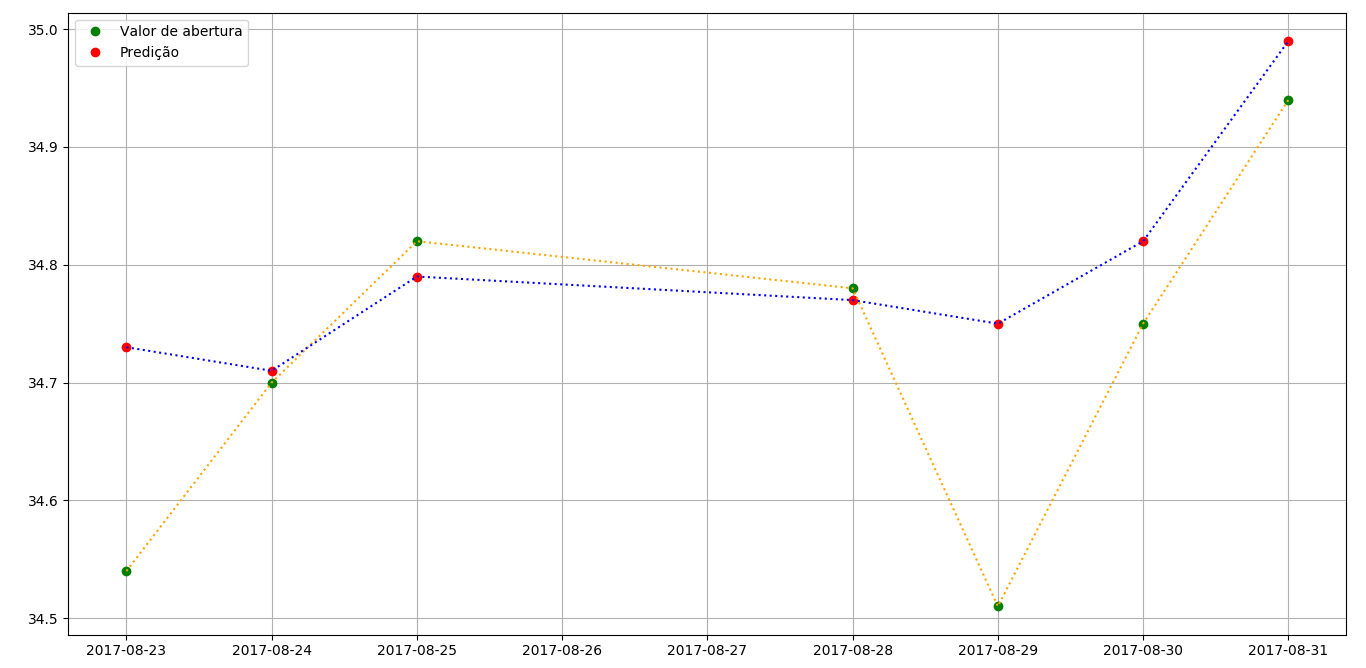
\includegraphics[width=1\textwidth]{predicao_intel}}
	\caption{Distribuição dos dados resultantes da RNA e seus valores esperados}
	\fonte{Elaborado pelo autor}
	\label{lingua}
\end{grafico}

Analisando o gráfico é possível observar como os resultados são próximos aos esperados. Os valores de abertura, nos respectivos dias testados, são representados por um ponto verde. Já os resultados obtidos pela rede são caracterizados pelo ponto vermelho. No Gráfico também fica evidente, de maneira ilustrativa, como a série não acompanhou as quedas do período e seguiu uma tendência crescente. 

\subsubsection{Treinamento com 1000 Iterações}	
Para comparar com a simulação anterior foi realizado um teste com 1000 épocas de treinamento, visando alcançar um resultado mais preciso e, também, validar se o aumento na quantidade de iterações, no processo de treinamento, melhoram os resultados retornados pela rede.

Para quantificar como ocorreu o processo de treinamento, basta multiplicar o número de iterações (1000) com o número de registros de testes (4117), resultando em um total de 4.117.000 exemplos calculados pela rede.
\begin{grafico}[h]
	\centering
	\fbox{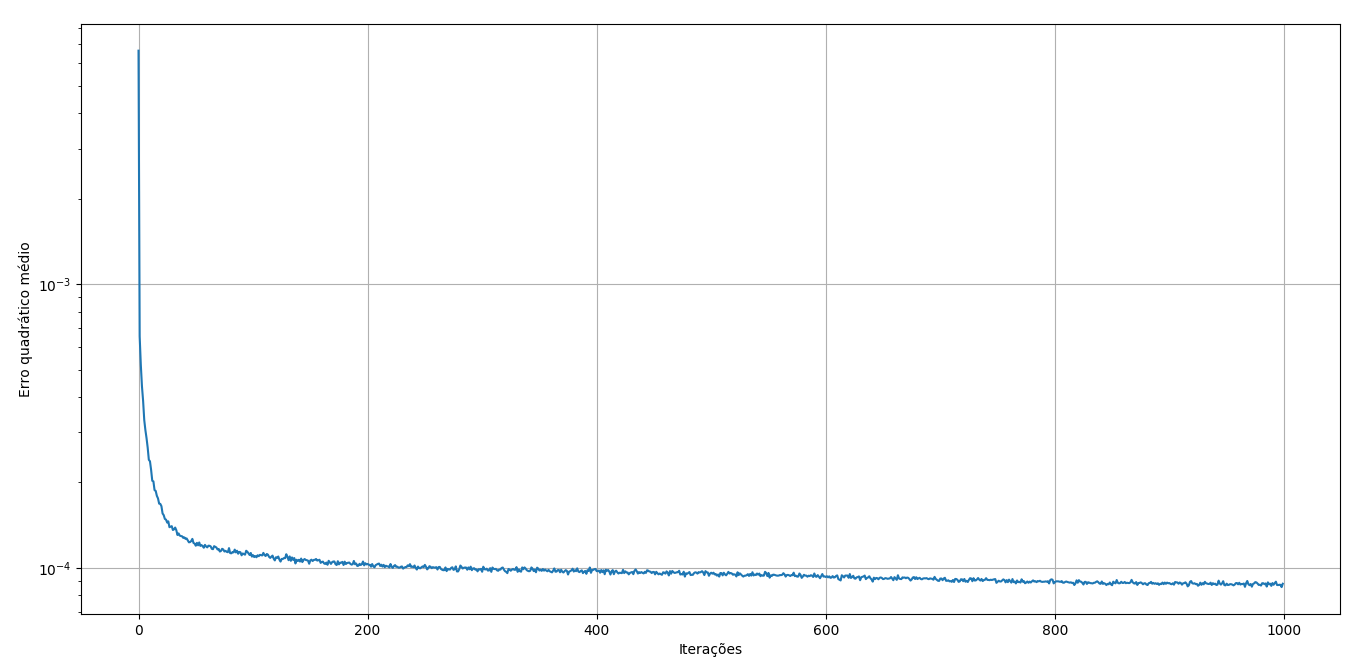
\includegraphics[width=1\textwidth]{erro_intel_1000iteracoes}}
	\caption{Decaimento do EQM no treinamento da rede}
	\fonte{Elaborado pelo autor}
	\label{lingua}
\end{grafico}

Para este cenário a rede iniciou-se, na primeira iteração, com um erro percentual de 0.00664064049629 e, após o término das 1000 épocas de treinamento, conclui-se com um erro percentual de 8.7943563121853531.$10^{-05}$. 

Analisando o Gráfico 10, pode-se observar que o erro obteve uma queda constante até 200 iterações, enquanto que, entre as iterações de número 200 até a de número 400, manteve o padrão com valores aproximados. Os últimos 600 ciclos mantiveram um decaimento mínimo do EQM.

Tendo em vista a simulação anterior, fica claro que a queda brusca e rápida aconteceria, pois a base de dados utilizada é a mesma, mas com um número maior de iterações, fazendo com que o EQM obtenha resultados mais baixos em comparação ao treino anterior.

O período para realizar os testes foi o mesmo utilizado na Tabela 1. Os dados foram devidamente refinados e normalizados e, a partir disto, foram ativados na rede. Os resultados obtidos são demonstrados na Tabela 3.
\begin{table}[h]
\centering
\caption{Resultados da predição realizada nos dados utilizados pela rede}
\vspace{0.5cm}
\begin{tabular}{>{\centering\arraybackslash}m{3cm} >{\centering\arraybackslash}m{3cm} >{\centering\arraybackslash}m{3cm} >{\centering\arraybackslash}m{3cm}}
\toprule
Data    & Valor esperado   & Resultado    & Erro (\%)\\
\midrule
23/08/2017 & 34.54 & 34.67 & 0.376\\
24/08/2017 & 34.70 & 34.64 & 0.172\\
25/08/2017 & 34.82 & 34.71 & 0.315\\
28/08/2017 & 34.78 & 34.68 & 0.287\\
29/08/2017 & 34.51 & 34.65 & 0.405\\
30/08/2017 & 34.75 & 34.70 & 0.143\\
31/08/2017 & 34.94 & 34.84 & 0.286\\
\bottomrule
\end{tabular}
\end{table}

Analisando a Tabela 3, pode-se observar que os resultados obtidos foram significativos, onde o percentual de erro calculado, através do erro relativo percentual, não ultrapassou a margem 0.50\%, se aproximando consideravelmente dos valores reais. Porém, a média de todo o período analisado obteve um erro de 0.28\%, superior ao treinamento anterior. O Gráfico 12 representa, de maneira ilustrativa, os resultados da série.
\begin{grafico}[h]
	\centering
	\fbox{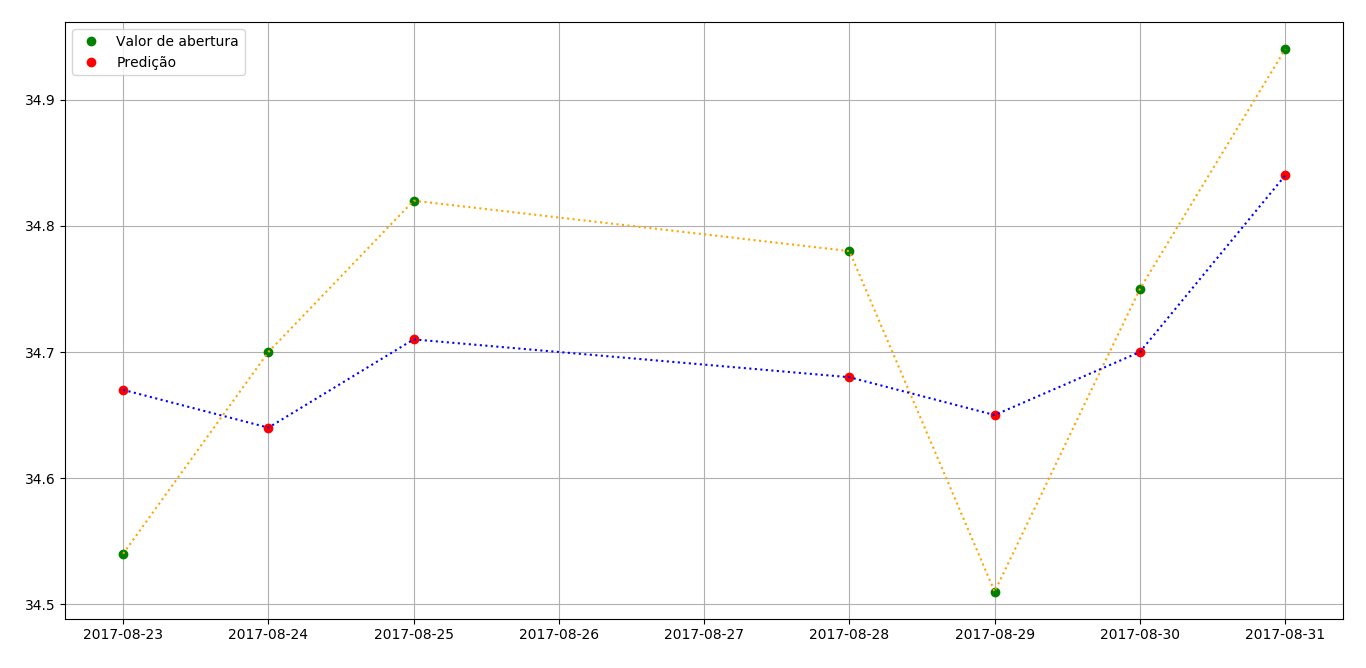
\includegraphics[width=1\textwidth]{predicao_intel_1000}}
	\caption{Distribuição dos dados resultantes da RNA e seus valores esperados}
	\fonte{Elaborado pelo autor}
	\label{lingua}
\end{grafico}

Apesar da diferença do erro percentual relativo entre os dois cenários ser de apenas 8\%, foi encontrada uma melhor parâmetrização para o presente modelo de dados utilizado em 200 iterações. Sendo assim, chega-se a definição que nem sempre um número maior de ciclos de treinamento aumentam a precisão da RNA. Neste caso, a rede sofreu uma convergência do EQM em torno de 200 iteraçoes, este detalhe pode ser observado visualizando o comportamento dos Gráficos 8 e 10. Dessa forma, as iterações posteriores propagaram o erro de forma desnecessária, alterando assim os pesos sinápticos dos neurônios e, automaticamente, causando uma maior dispersão nos resultados. Este processo ocorrido na segunda simulação, na literatura, é denominado \textit{Overtraining}, detalhado no Capítulo 3.